\documentclass[envcountsect,dvips]{beamer}

\setbeamertemplate{background canvas}[vertical shading][bottom=yellow!20,top=blue!10]
%\usetheme{Darmstadt}
\usetheme{Warsaw}
%\usefonttheme[onlysmall]{structurebold}

\usepackage{natbib}
\usepackage{bibentry}
\bibliographystyle{plain}
\usepackage{chngcntr}

\usepackage[utf8]{inputenc}
\usepackage{default}
\usepackage{amsmath}
\usepackage{amsfonts}
\usepackage{amssymb}

\usepackage{graphicx}
\usepackage{caption}
\usepackage{subcaption}

\usepackage{color,xcolor,ucs}% para textcolor

%http://alumni.cs.ucr.edu/~saha/stuff/memaddr.html

%%%%%%%%%%%%%%%%%%%%%%%%%%%%%%%%%%%%%%%%%%%%%%%%%%%%%%%%%%%%%%%%%%%%%%%%%%
\begin{document}

\title[Memoria virtual:   ] % (optional, only for long titles)
{Memoria virtual:}
\subtitle{Paginação, segmentação - endereçamento}
\author[Fernando] % (optional, for multiple authors)
{Fernando Pujaico Rivera\inst{1}}
\institute[Universidade Federal de Lavras] % (optional)
{
  \inst{1}%
  Universidade Federal de Lavras
}
\date[2016] % (optional)
{Aula-1 2016}
\subject{Computer Science}
\frame{\titlepage}

%%%%%%%%%%%%%%%%%%%%%%%%%%%%%%%%%%%%%%%%%%%%%%%%%%%%%%%%%%%%%%%%%%%%%%%%%%%%%%%%
%%%%%%%%%%%%%%%%%%%%%%%%%%%%%%%%%%%%%%%%%%%%%%%%%%%%%%%%%%%%%%%%%%%%%%%%%%%%%%%%
%%%%%%%%%%%%%%%%%%%%%%%%%%%%%%%%%%%%%%%%%%%%%%%%%%%%%%%%%%%%%%%%%%%%%%%%%%%%%%%%
\section{Memoria Virtual}
%%https://www.youtube.com/watch?v=X0XscX9ugp0

\begin{frame}{Memoria física \cite{arq}}
\begin{figure}
\centering
\includegraphics[width=10cm]{images/memoriavirtual0.eps}
\caption{Como se usa a memoria física}
\label{fig:memoria0}
\end{figure}
\end{frame}

\begin{frame}{Memoria física e memoria virtual}
\begin{figure}
\centering
\includegraphics[width=10cm]{images/memoriavirtual.eps}
\caption{Como se usa a memoria virtual}
\label{fig:memoria}
\end{figure}
\end{frame}

\begin{frame}{Memoria virtual}
\begin{minipage}{4.5cm}
\begin{figure}
\centering
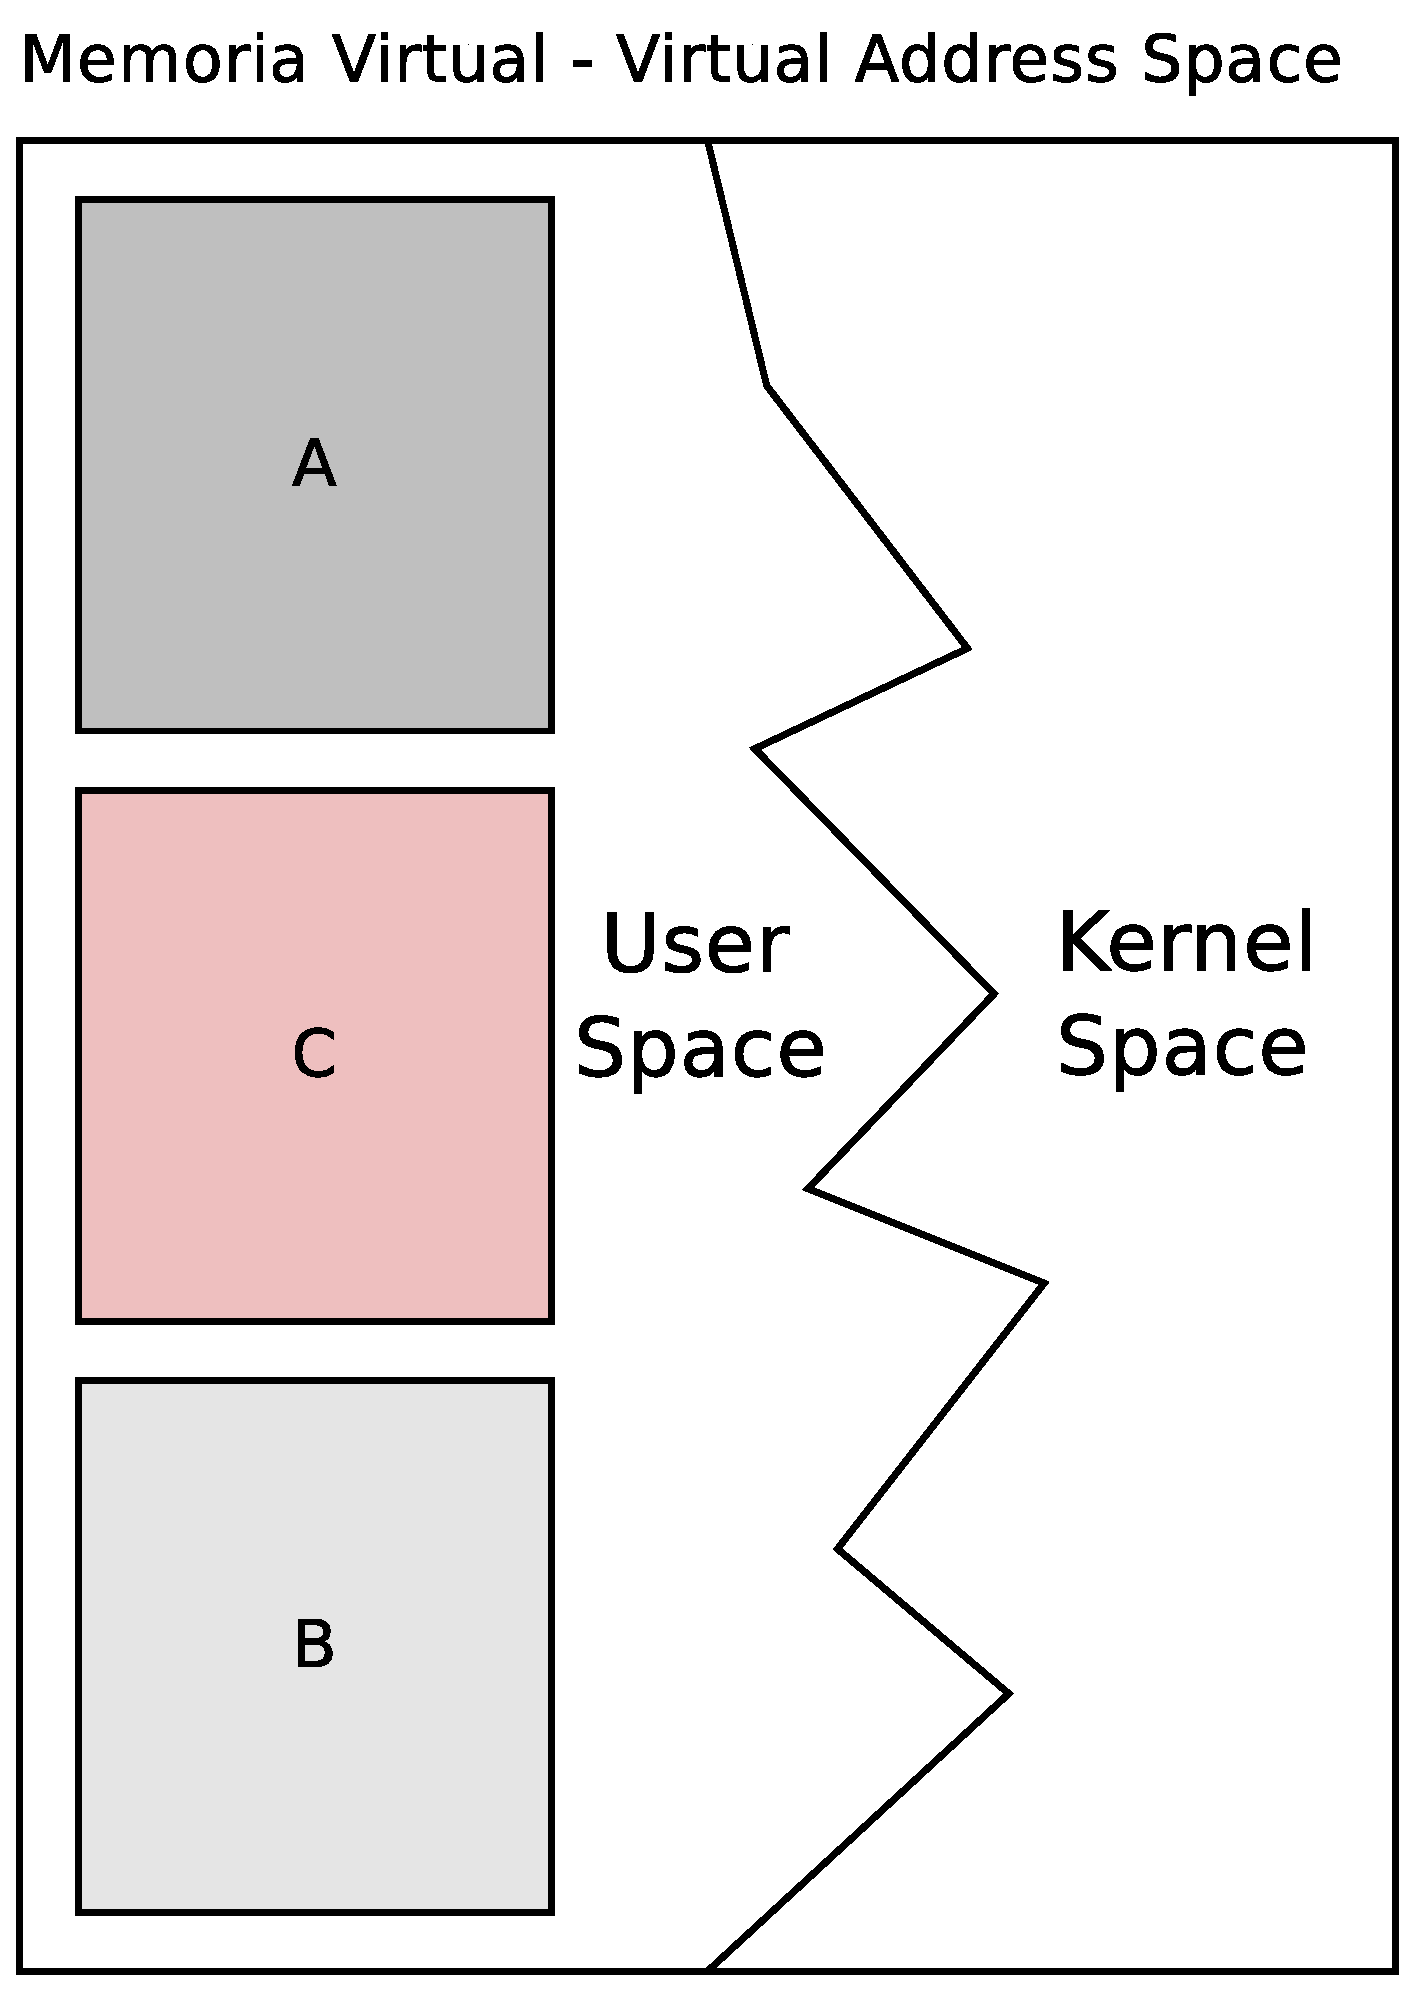
\includegraphics[width=4cm]{images/memoriavirtual2.eps}
%\caption{Como se usa a memoria virtual}
\label{fig:memoria}
\end{figure}
\end{minipage}
\begin{minipage}{6cm}



\begin{tabular}{ l || r | r }
  \hline			
  ~            & User S. & Kernel S. \\
  \hline			
  Linux 32-bit \cite{VIRTUAL}  & 3GB & 1GB \\
  Win. 32-bit                  & 2GB & 2GB \\
  \hline		
  Linux 64-bit \cite{linux64}  & 128TB & 128TB \\
  W10 64-bit                   &   8TB &   8TB \\  
  W8S 64-bit   \cite{win64}  & 128TB & 128TB \\  
  \hline  
\end{tabular}
\end{minipage}
\end{frame}


\begin{frame}
CPUs de arquitetura x86-64, ou seja, o AMD Athlon 64 \cite{AMD64}

~\\
~\\

\begin{tabular}{r | l | l}
~                & 32-bits & 64-bits\\
\hline \hline
 End. de Mem. virtual   & 32-bits & 48-bits $\equiv$ 2 regiões de 47-bits\\ 
 \hline  
 End. de Mem. real (RAM)& 30-bits & 40-bits \cite{AMD64}\\
 \hline 
\end{tabular}

~\\

\begin{minipage}{6cm}
\begin{figure}
\centering
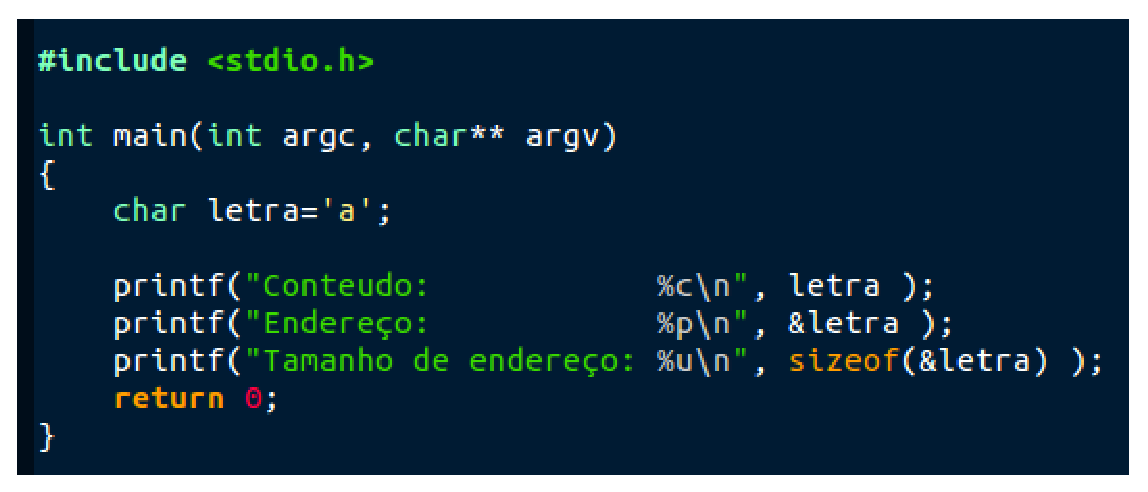
\includegraphics[width=\textwidth]{cfiles/test.eps}
%\caption{Segmentação (compilador) e paginação}
\label{fig:test1}
\end{figure}
\end{minipage}
\begin{minipage}{4.5cm}
Conteúdo: a\\
Endereço: 0x7ffd 3e55 fabf\\
Tam. endereço: 8 Bytes
\end{minipage}

\end{frame}


%http://cameraweb.ccuec.unicamp.br/watch_video.php?v=cw0dY0cb2y#
\begin{frame}{Segmentação e paginação}
\begin{figure}
\centering
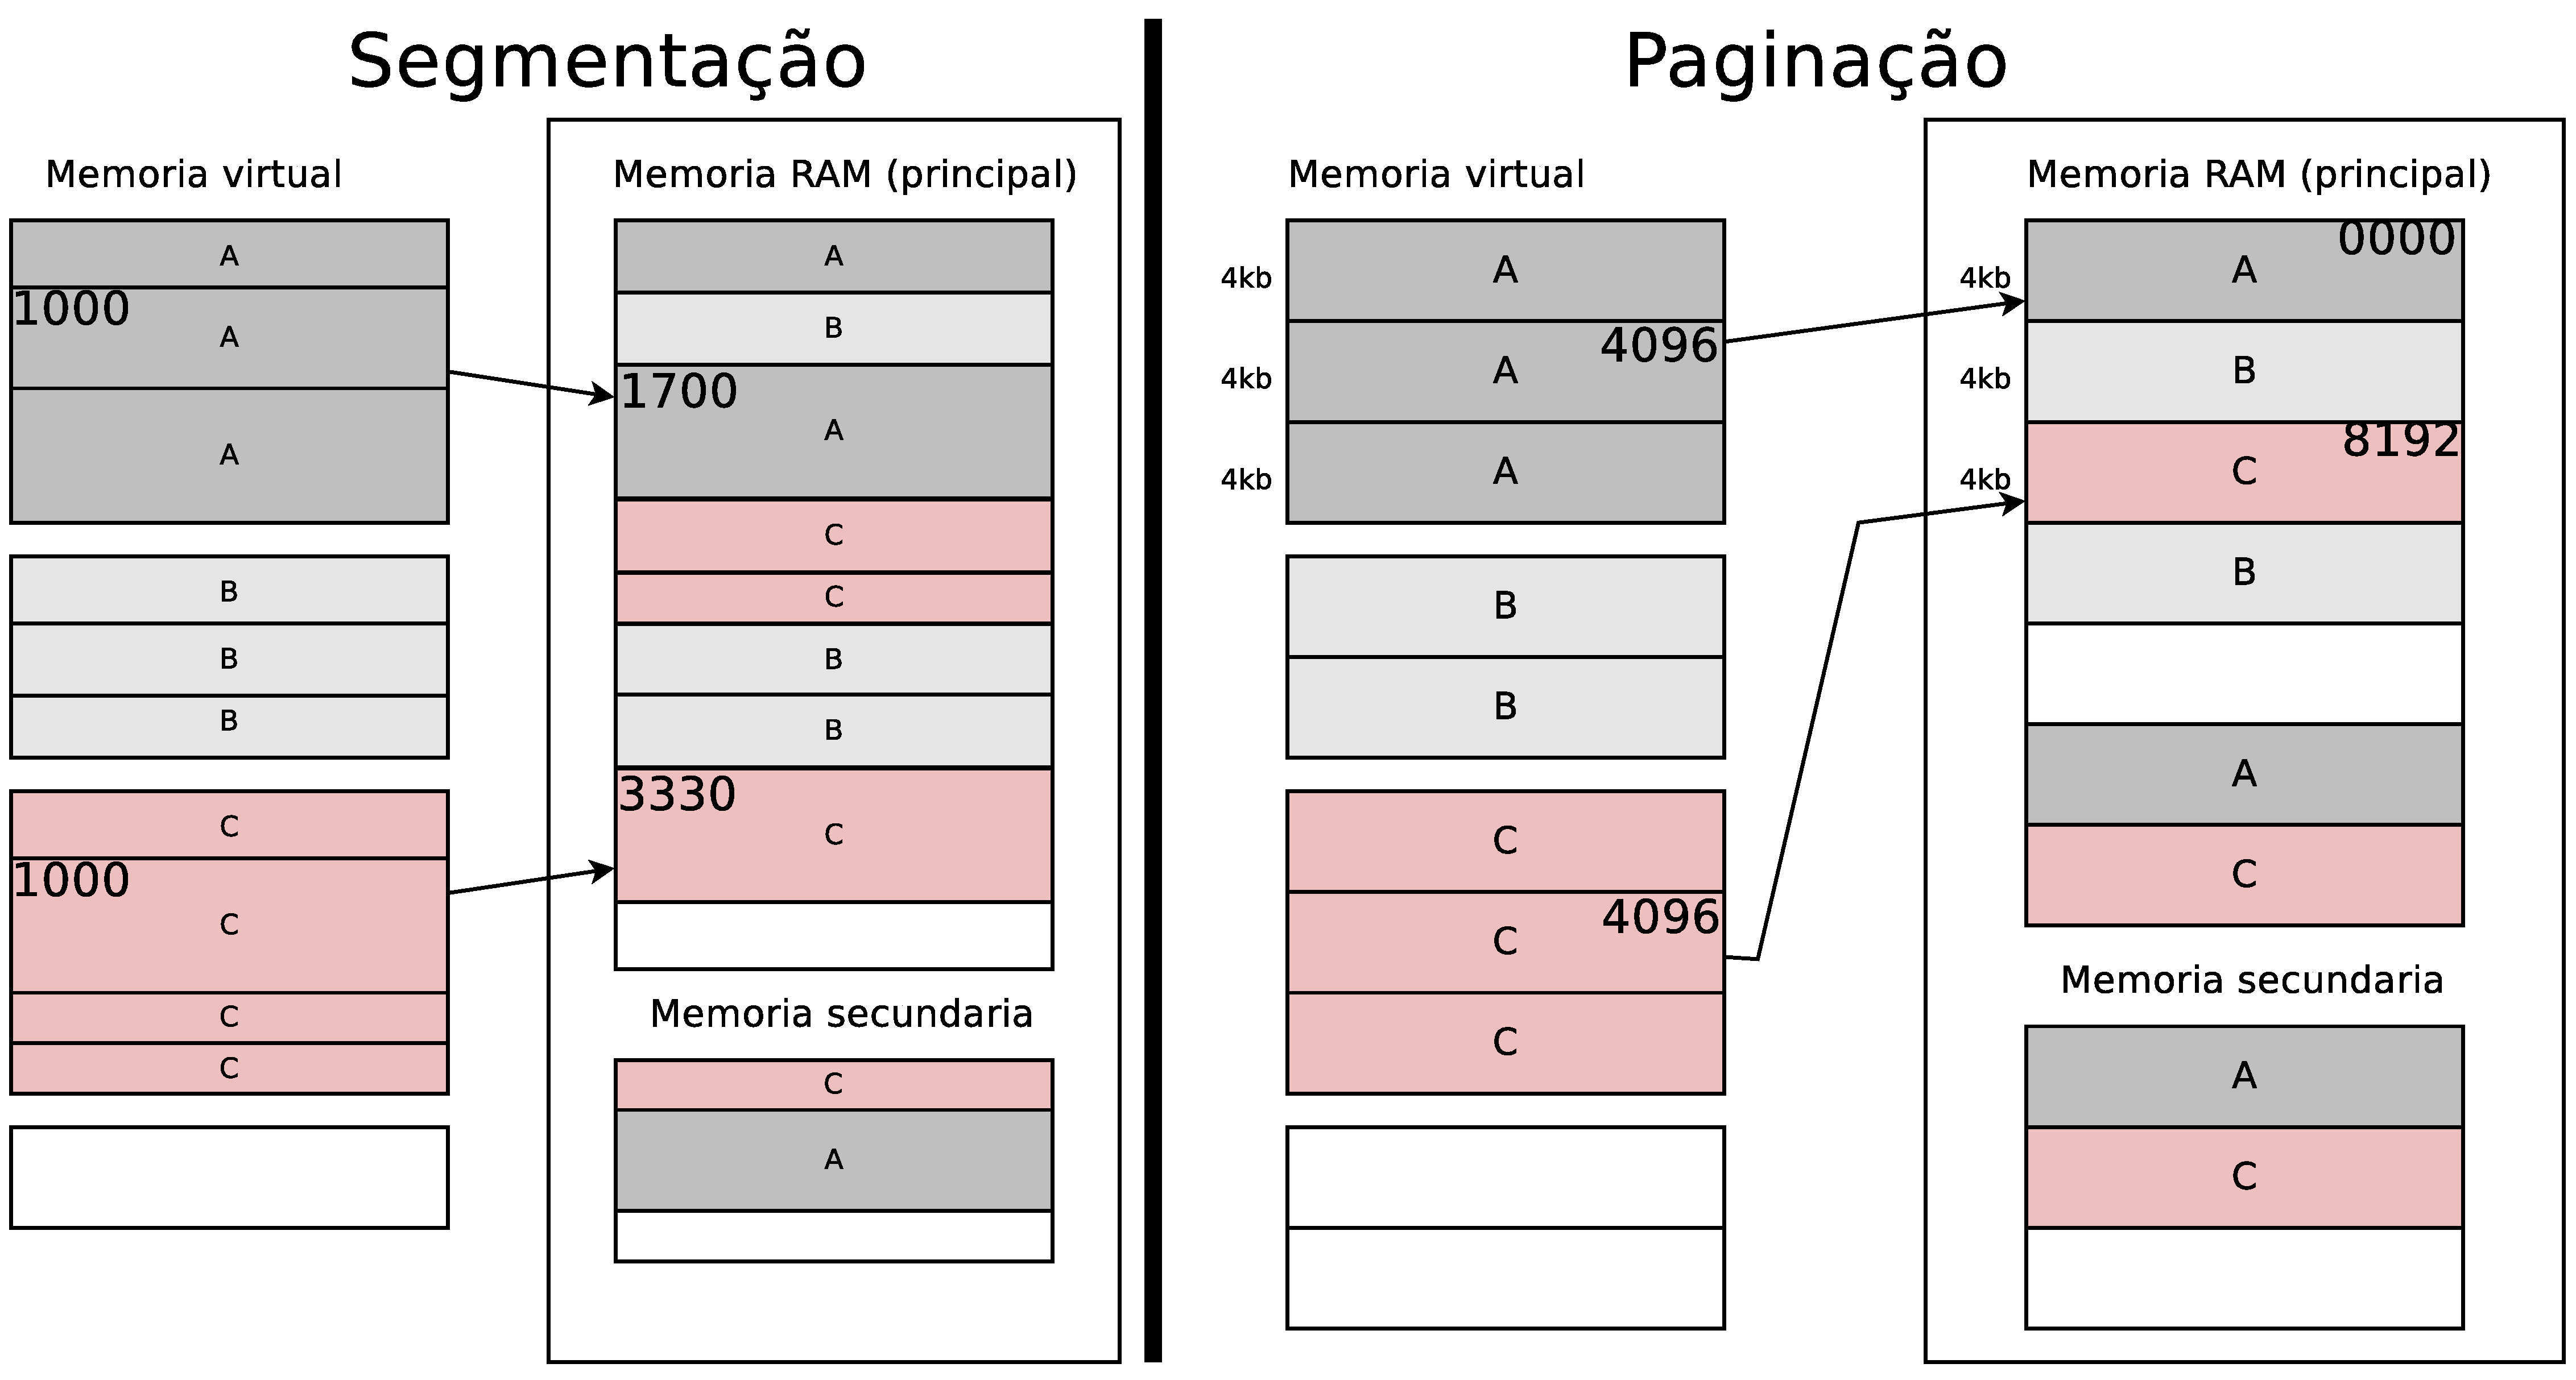
\includegraphics[width=10cm]{images/segmentpage.eps}
\caption{Segmentação (compilador) e paginação}
\label{fig:segmentpage}
\end{figure}
\end{frame}

\begin{frame}{Endereçamento}
Na arquitetura x86 ({\color{red}32} e {\color{blue}64} bits), são usadas a segmentação e a paginação
\begin{figure}
\centering
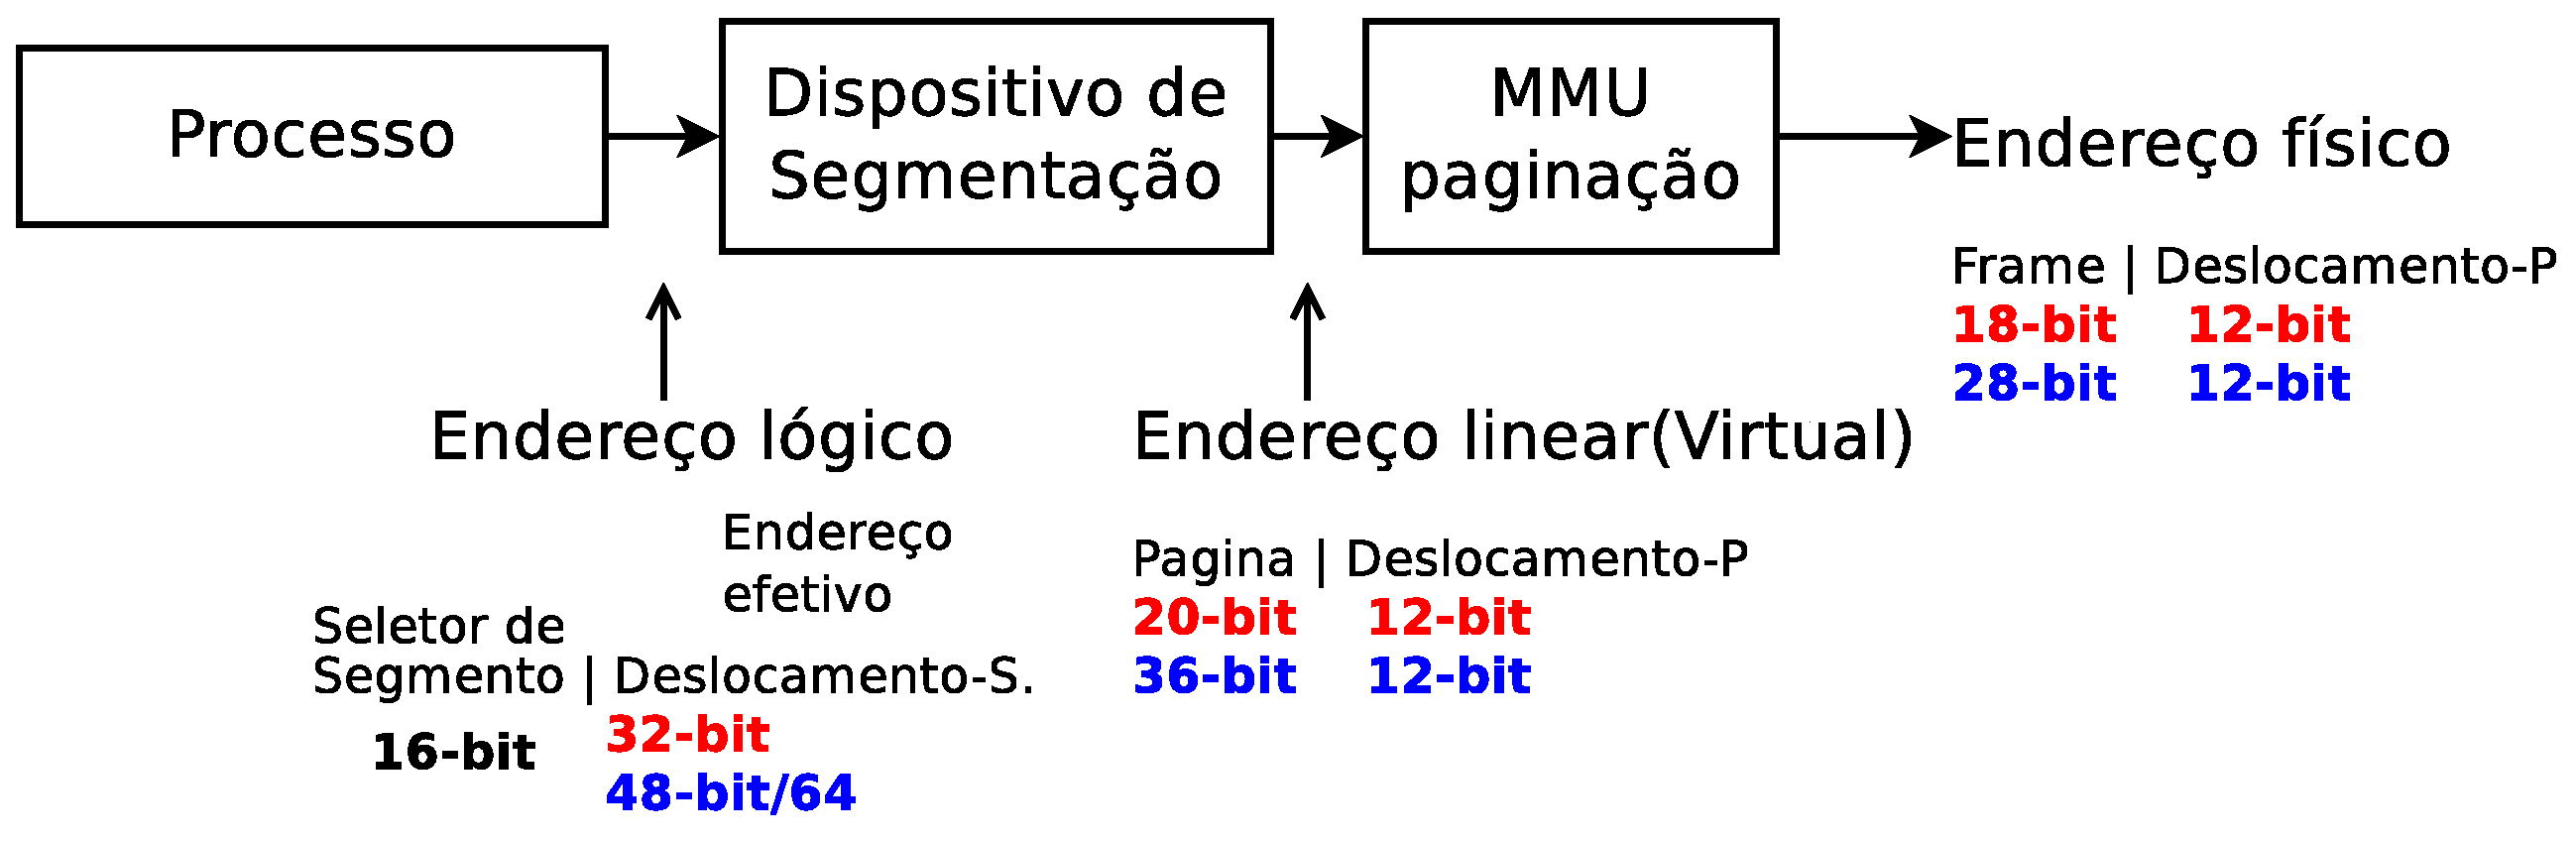
\includegraphics[width=10cm]{images/enderecamento.eps}
%\caption{Segmentação e paginação}
\label{fig:enderecamento}
\end{figure}
12-bit gera 4kB espaços de memoria.
\end{frame}

\begin{frame}{Endereçamento}
\begin{figure}
\centering
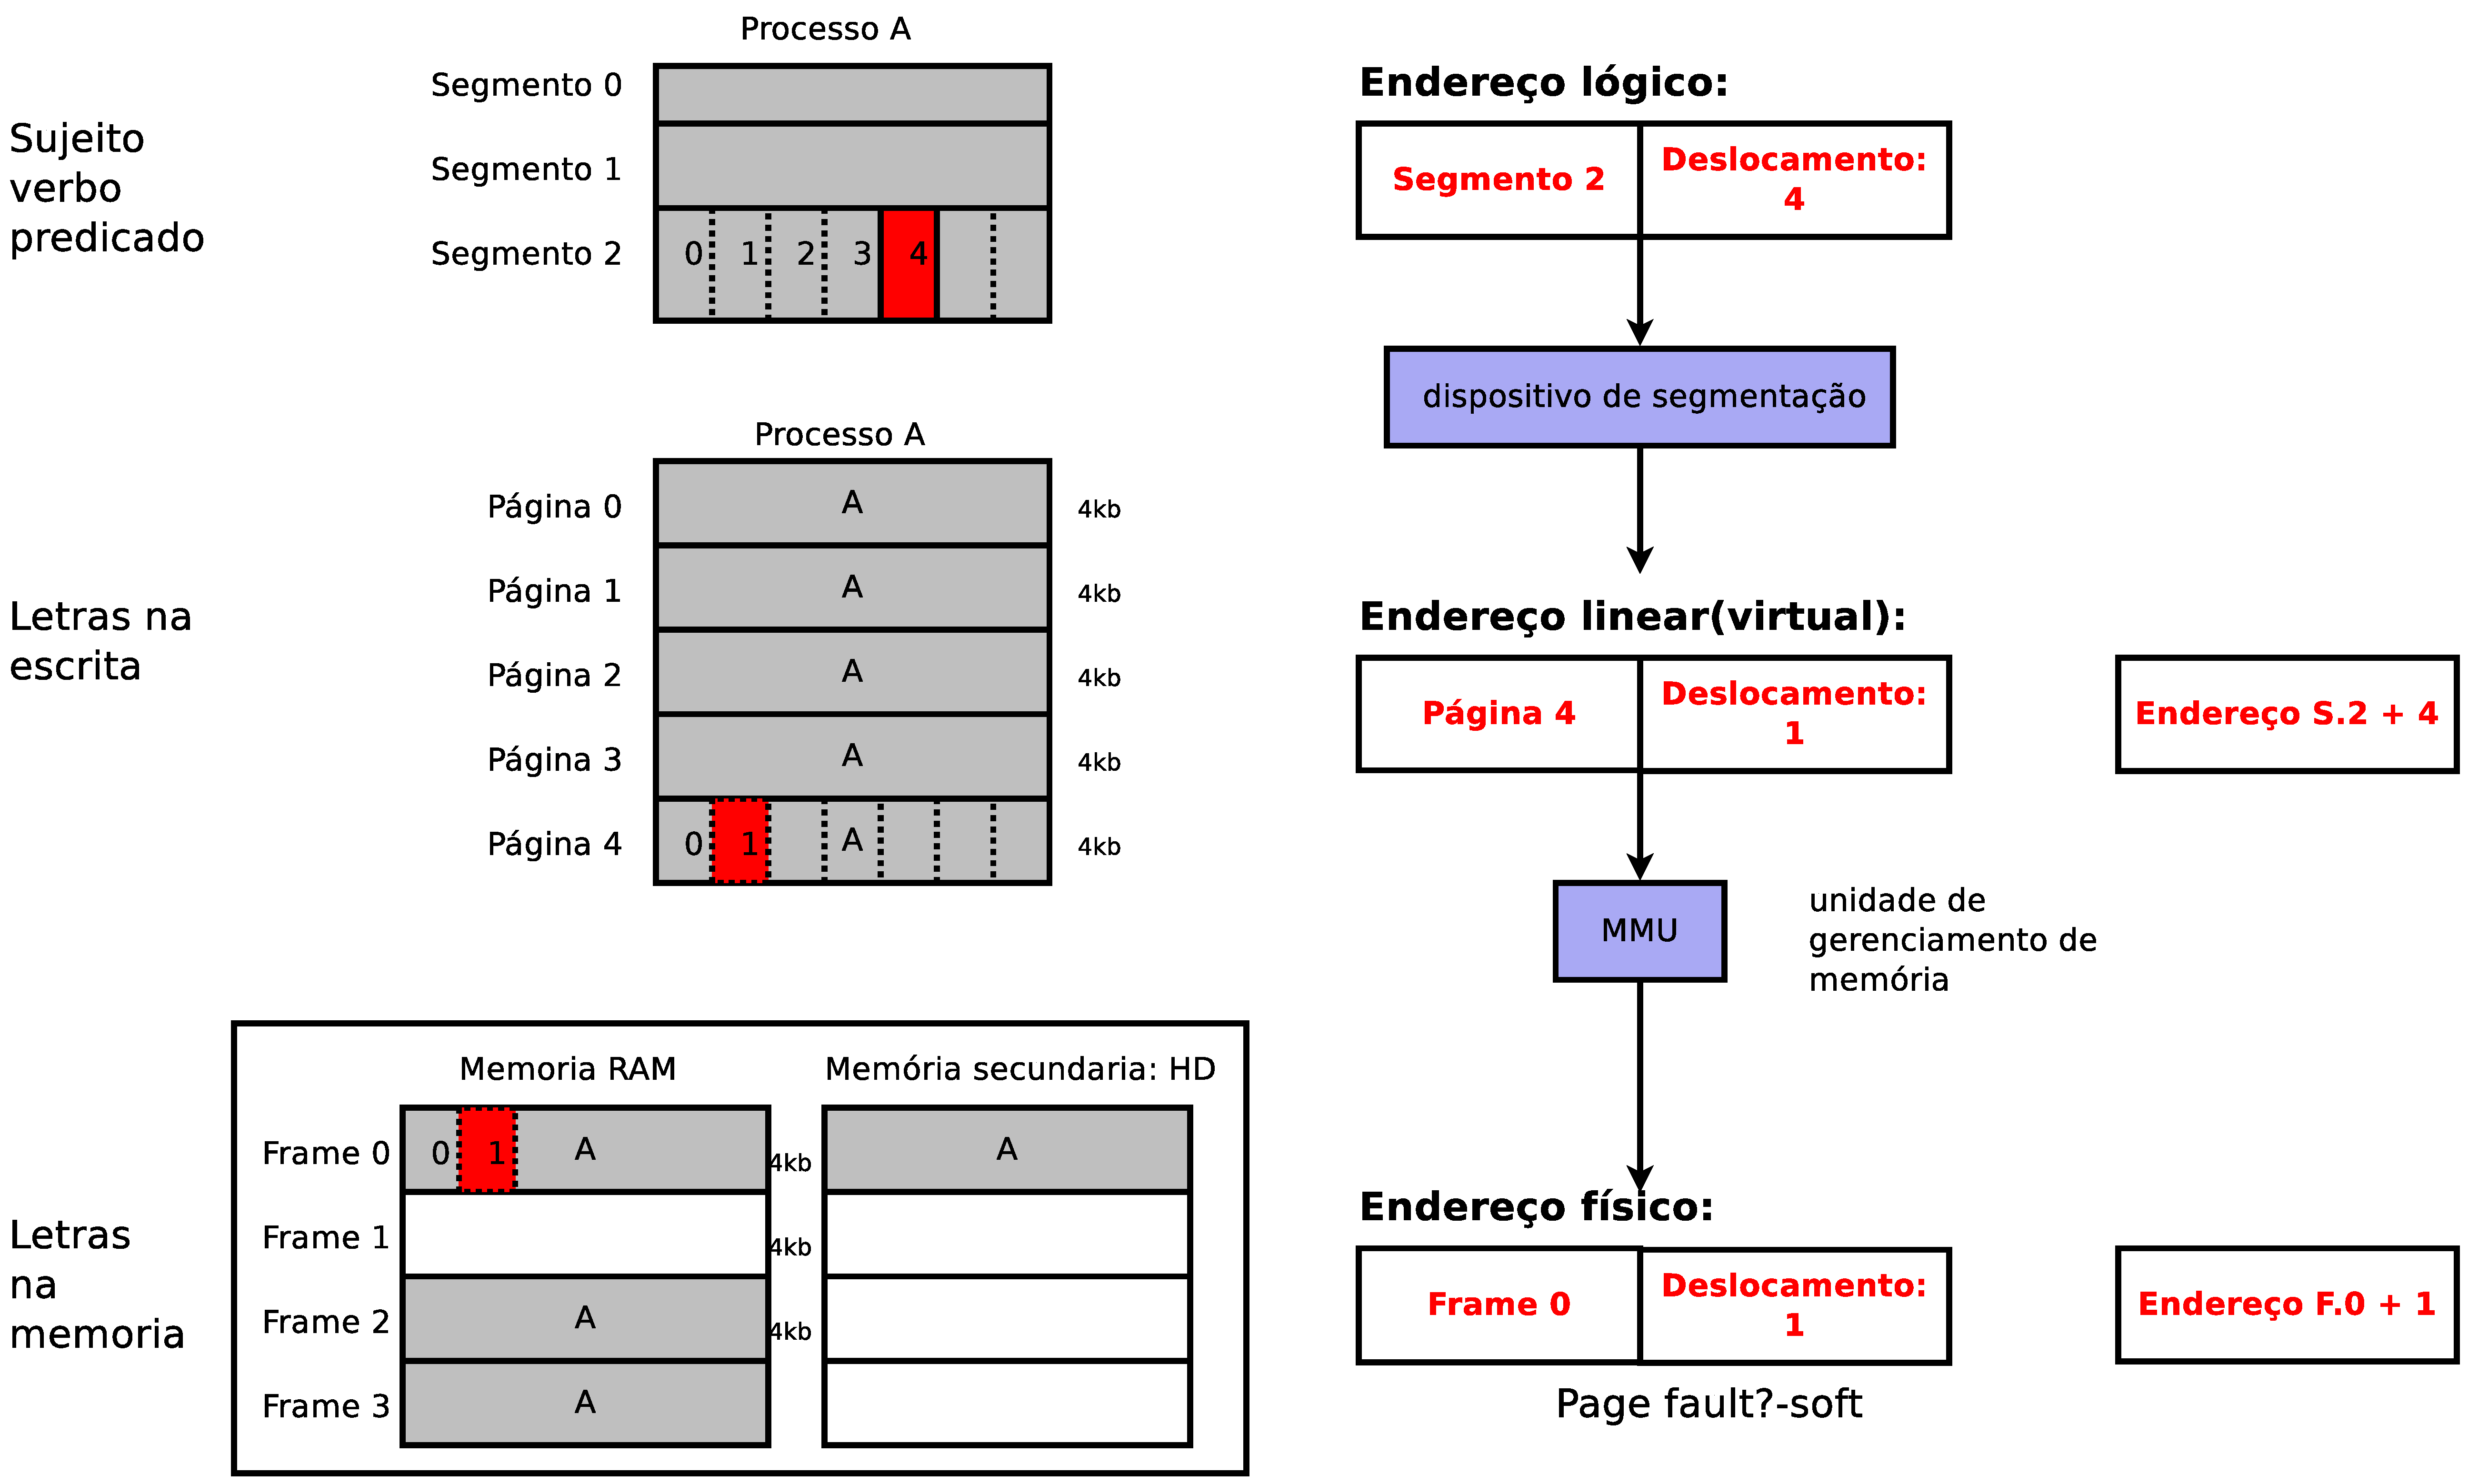
\includegraphics[width=10.5cm]{images/enderecamento2.eps}
%\caption{Segmentação e paginação}
\label{fig:enderecamento2}
\end{figure}
\end{frame}

\begin{frame}{Endereçamento}
\begin{figure}
\centering
\includegraphics[width=10.5cm]{images/addressing.eps}
%\caption{Segmentação e paginação}
\label{fig:addressing}
\end{figure}
\end{frame}

%%https://www.youtube.com/watch?v=d11U38UzfOY
%https://www.youtube.com/watch?v=hvZWjigTWOQ
\begin{frame}{Endereço lógico $\rightarrow$ endereço linear}
\begin{figure}
\centering
\includegraphics[width=9.5cm]{images/segmento.eps}
%\caption{Segmentação e paginação}
\label{fig:pagina}
\end{figure}
\end{frame}

%%https://www.youtube.com/watch?v=d11U38UzfOY
%https://www.youtube.com/watch?v=hvZWjigTWOQ
\begin{frame}{Endereço lógico $\rightarrow$ endereço linear}
\begin{figure}
\centering
\includegraphics[width=9.5cm]{images/segmento2.eps}
%\caption{Segmentação e paginação}
\label{fig:pagina}
\end{figure}
\end{frame}

%%https://www.youtube.com/watch?v=d11U38UzfOY
\begin{frame}{Endereço linear $\rightarrow$ endereço físico}
\begin{figure}
\centering
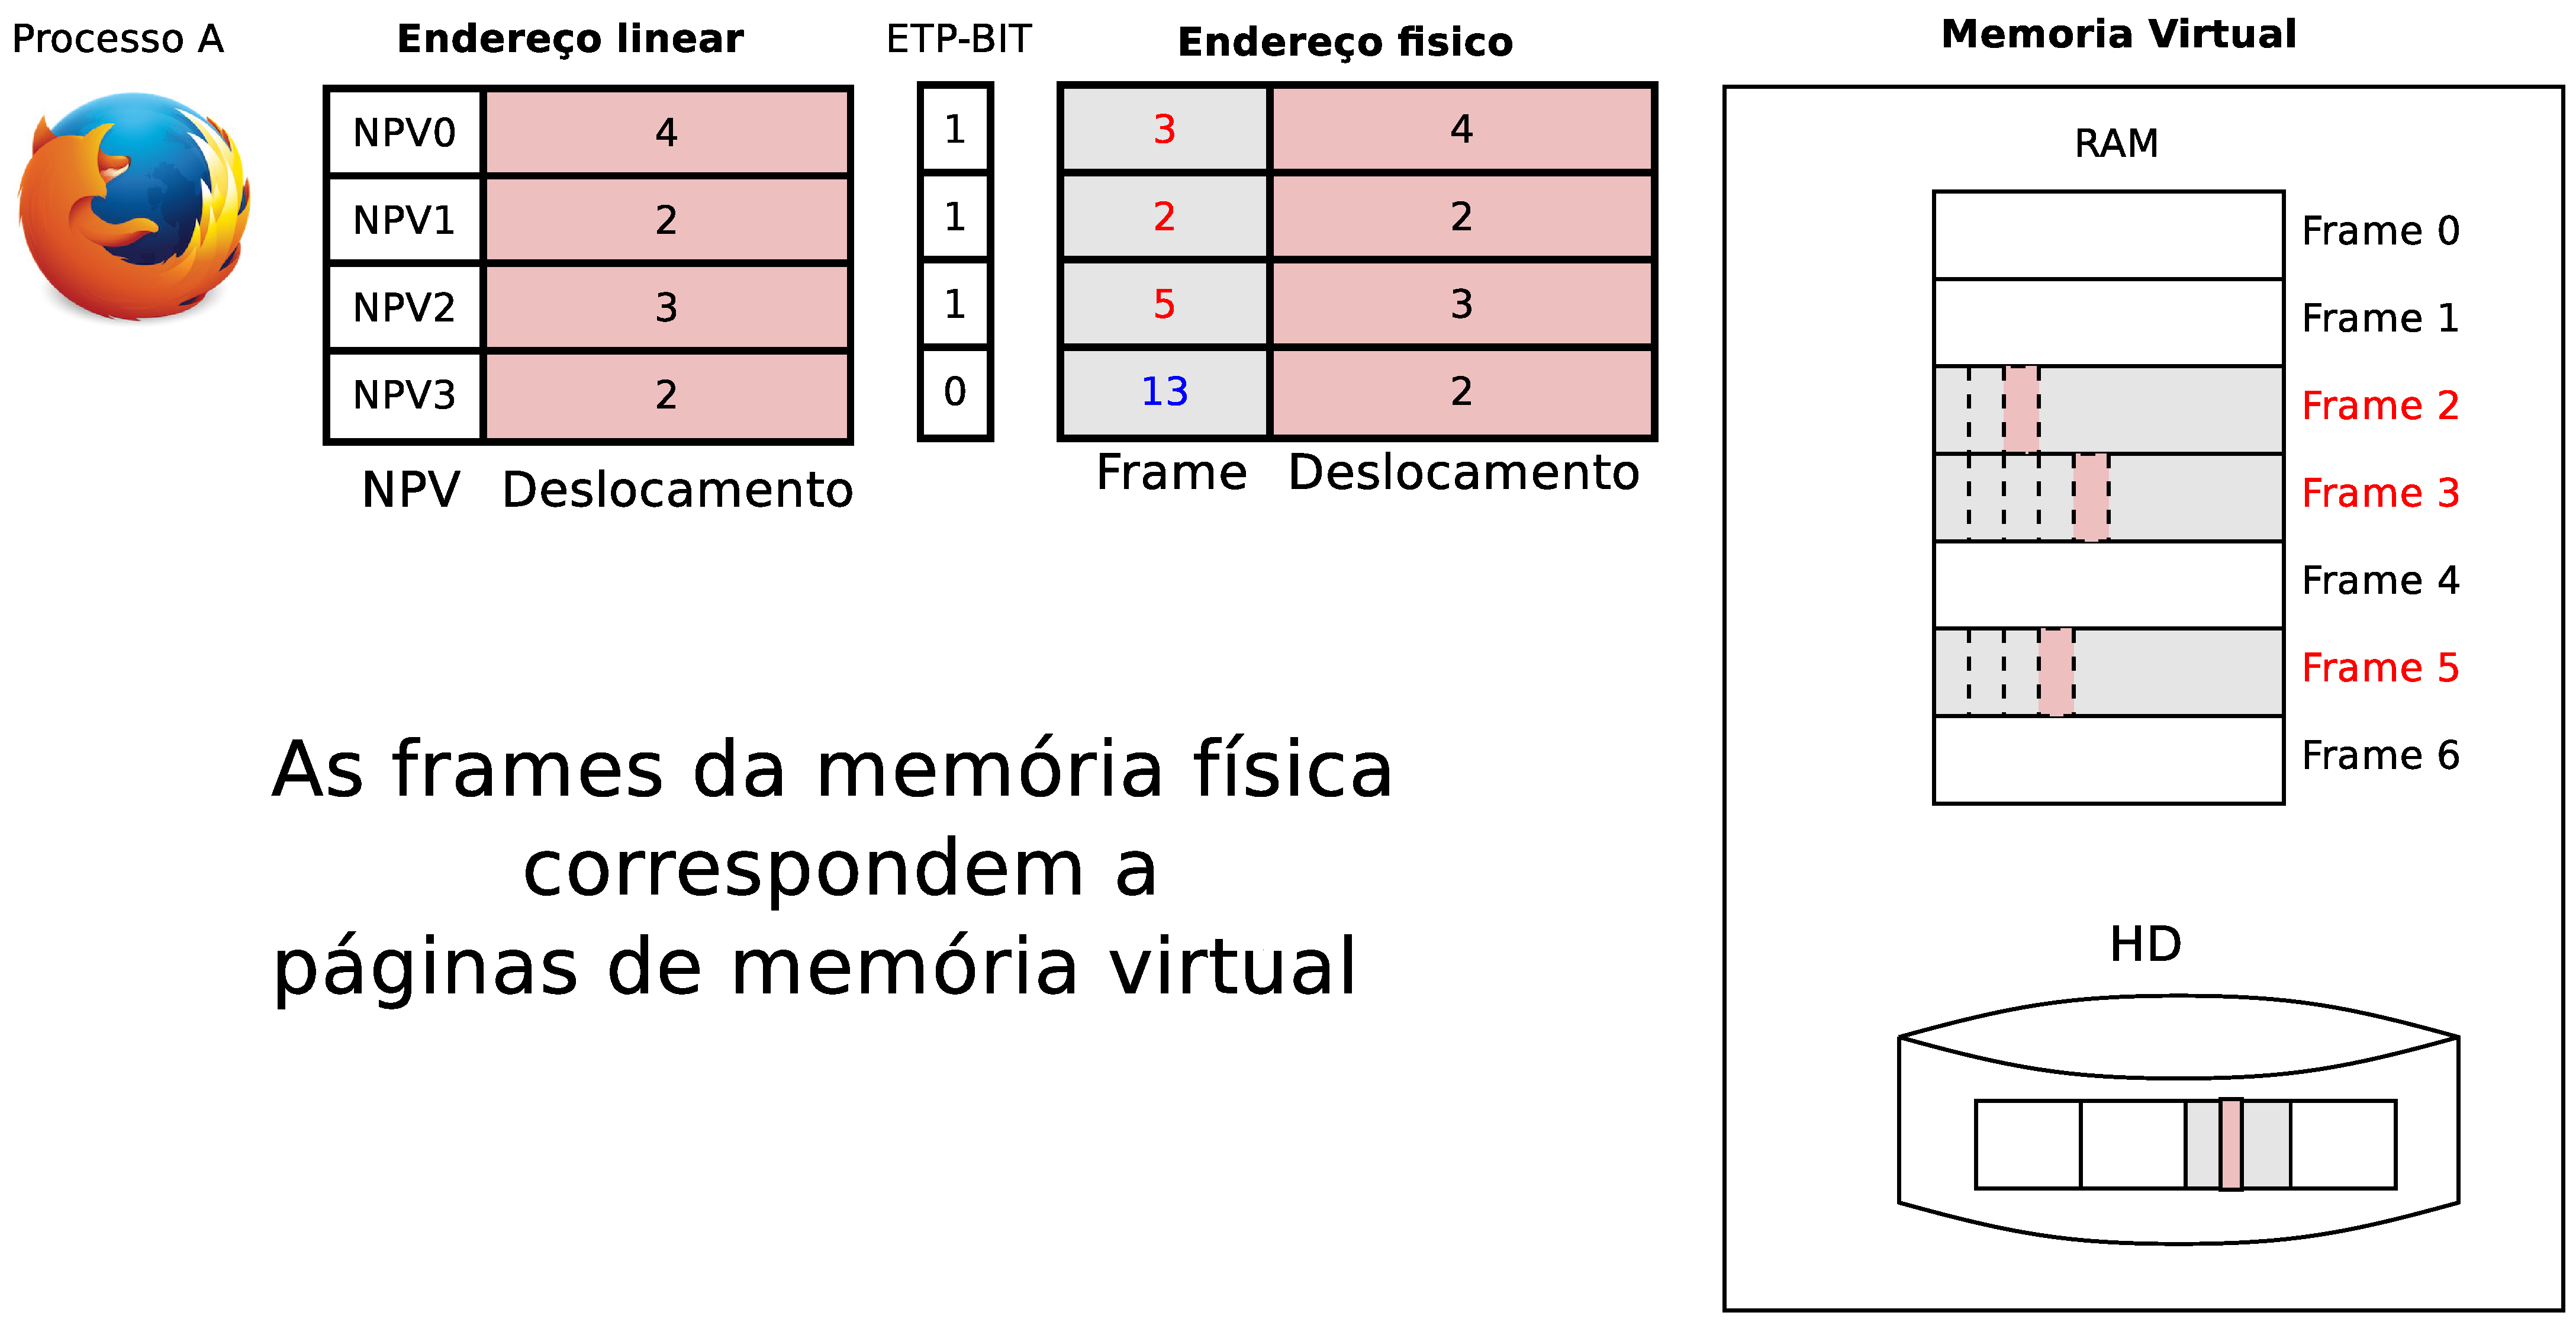
\includegraphics[width=9cm]{images/pagina.eps}
%\caption{Segmentação e paginação}
\label{fig:pagina}
\end{figure}
\end{frame}

\begin{frame}{Endereço linear (Virtual) $\rightarrow$ endereço físico}
\begin{figure}
\centering
\includegraphics[width=10cm]{images/pagina2.eps}
%\caption{Segmentação e paginação}
\label{fig:pagina2}
\end{figure}
\end{frame}

\begin{frame}{Segmentação e paginação}
\begin{minipage}{.45\textwidth}
Segmentação:
\begin{itemize}
 \item Dividido (segmentos) analisando sua estrutura logica.
 \item Vários processos podem usar partes de um mesmo segmento.
  \item Uso de espaços livres entre segmentos.
  \item Segmento com níveis de privilégios de acesso.
\end{itemize}
\end{minipage}
\begin{minipage}{.45\textwidth}
Paginação:
\begin{itemize}
 \item pedaços de memoria de tamanho fixo (4kB).
 \item Sem níveis de privilégios de acesso.
 \item paginas são mais pequenas que os segmentos.
\end{itemize}
~\\
~\\
\end{minipage}%
\end{frame}

\section{Administração da memoria}
\begin{frame}{Administração da memoria virtual pelo S.O.}

Os dados usados de forma continua estão na memoria física.
\begin{description}
  \item[Politicas de carga (fetch)] Quando trazer uma pagina/segmento
  à memoria física  (DEMANDA Vs. Anticipada)
  \item[Politicas de colocação (placement)] Onde por a pagina/segmento
  na memoria física
  \item[Politicas de substituição (Replacement) ] Quando a memoria RAM está cheia \ldots
\end{description}

\end{frame}


%% http://www.geeksforgeeks.org/memory-layout-of-c-program/
%% http://alumni.cs.ucr.edu/~saha/stuff/memaddr.html


%%%%%%%%%%%%%%%%%%%%%%%%%%%%%%%%%%%%%%%%%%%%%%%%%%%%%%%%%%%%%%%%%%%%%%%%%%%%%%%%
\begin{frame}[allowframebreaks]
        \frametitle{References}
        \bibliographystyle{plain}
\bibliography{memoriavirtual}
\end{frame}



\end{document}
